\documentclass{article}
\usepackage{packages}
\usepackage[utf8]{inputenc}
\usepackage[T1]{fontenc}
\usetikzlibrary{shapes.geometric}

\begin{document}

\section{Electrons I (FEG)}

\subsubsection*{(a)}
For a system at temperature $T$ the free energy is given by 
\begin{equation*}
    G(p, T) = E + pV - TS
    \label{eq:FreeEneergy}
\end{equation*}
where the pressure $p$, the volume $V$ and the temperature $T$ are connected through a state equation of the type $\phi(p, V, T) = 0$ that depends
on the system. \\
For $T=0$ equation \ref{eq:FreeEneergy} reduces to
\begin{equation}
    G(p, T) = E + pV
\end{equation}
where $E$ is the energy of the system. \\
In the Free Fermi Electron Gas model the energy can be computed as
\begin{equation}
    E(T) = \int_{E_{min}}^{E_{max}} d\epsilon \ DOS(\epsilon) \ f_{FD}(\epsilon, T) \ \epsilon 
\end{equation}
where $f_{FD}(\epsilon)$ is the Fermi-Dirac distribution 
\begin{equation*}
    f_{FD}(\epsilon) = \frac{1}{e^{(\epsilon_i - \mu)/k_B T} + 1}
\end{equation*}
and indicates the average number of fermions in a single-particle state. \\
In the limit of zero temperature one gets
\begin{equation}
    \lim_{T \to 0} E(T) = \int_{E_{min}}^{E_{max}} d\epsilon \ \lim_{T \to 0} \ DOS(\epsilon) \ f_{FD}(\epsilon, T) \ \epsilon
    \label{eq:energy_FEFG}
\end{equation}
The 3D density of states function 
\begin{equation}
    DOS(\epsilon) = \frac{V}{2\pi^2} \ \left(\frac{2m}{\hbar^2}\right)^{3/2} \ \epsilon^{1/2}
\end{equation}
does not depend on the temperature, while the Fermi-Dirac distribution function in the limit $T \to 0$ reduces to 
\begin{equation}
    \lim_{T \to 0} f_{FD}(\epsilon) = 
    \begin{cases}
        1 \qquad \text{if } \epsilon < \mu \\
        \frac{1}{2} \qquad \text{if } \epsilon = \mu \\ 
        0 \qquad \text{if } \epsilon > \mu
    \end{cases}
\end{equation}
so that \ref{eq:energy_FEFG} becomes 
\begin{equation*}
    E \equiv E(T=0) = \frac{V}{2\pi^2} \ \left(\frac{2m}{\hbar^2}\right)^{3/2} \int_{E_{min}}^{E_{max}} \epsilon^{3/2} \, d\epsilon
\end{equation*}
In the last integral the extrema are $E_{min} = 0$ and $E_{max} = \epsilon_F$,. $E_F$ is the Fermi energy which is, by definition, the energy of 
the last occupied state. Hence
\begin{equation}
    E = \frac{V}{5\pi^2} \ \left(\frac{2m}{\hbar^2}\right)^{3/2} \, \epsilon_F^{5/2}
    \label{eq:energy_energyfermi}
\end{equation}
and using the relation 
\begin{equation*}
    \epsilon_F = \frac{\hbar^2}{2m} \left(\frac{3\pi^2N}{V}\right)^{1/3}
\end{equation*}
one obtains
\begin{equation*}
    E = \frac{V}{5\pi^2} \ \left(\frac{2m}{\hbar^2}\right)^{3/2} \, \epsilon_F^{5/2}
\end{equation*}
The pressure can then be calculated by the Maxwell relation 
$$p = -\frac{\partial E}{\partial V} = \frac{2}{3} \ \frac{1}{5\pi^2 V^{2/3}} \ \frac{\hbar^2}{2m} (3\pi^2N)^{5/3} = \frac{2}{3}\frac{E}{V}$$
so that 
$$G = E + pV = \frac{5}{3} E = \frac{2}{3} \frac{V}{5\pi^2} \ \left(\frac{2m}{\hbar^2}\right)^{3/2} \ \epsilon^{5/2}$$
which can be rearranged as
$$G = N \epsilon_F$$
Equating this result to the formula given in the text of the exercise $G = N\mu$ one concludes that at temperature $T=0$ 
\begin{equation}
    \epsilon_F = \mu
\end{equation}

\subsubsection*{(b)}
By looking at figure \ref{fig:fFD_mu}, one can notice that for $T=0.01 \, T_F$ and $T=0.1 \, T_F$ (blue and green lines) the dashed curves overlap with the continuous lines. This means that the approximation 
$\mu = \epsilon_F$ in the Fermi-Dirac distribution is legitimate. On the other side for $T=T_F/2$ one can see that the dashed line does not overlap with the continous one and in particular the maximum difference 
occurs at $\epsilon = \epsilon_F$, where the approximated function ($\mu = \epsilon_F$) is always $1/2$ and the true function is not. This means that the approximation is not anymore valid.
\begin{figure}[htp]
    \centering 
    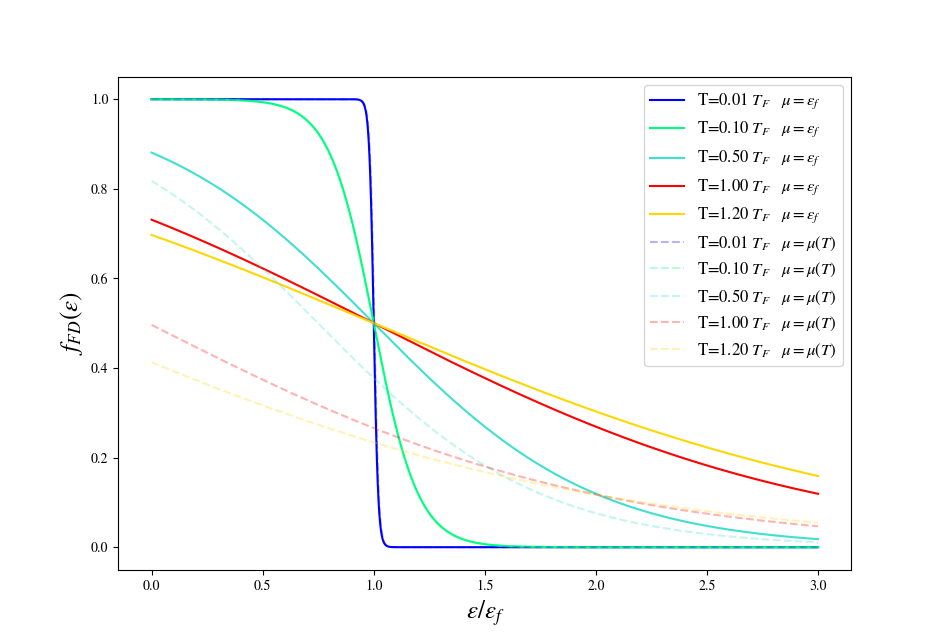
\includegraphics[scale=0.5]{scripts/f_fd_mu.png}
    \caption{Fermi-Dirac distribution for various temperature values. The continous lines correspond to 
    the distribution drawn by keeping the chemical potential constant at $\mu=_{epsilon_F}$, while the dashed lines represent the true relations.}
    \label{fig:fFD_mu}
\end{figure}

\subsubsection*{(c)}
The number of orbitals whose energy is less than or equal to $\epsilon$ is given by 
\begin{equation}
    N = \frac{V}{3\pi^2} \left(\frac{2m\epsilon}{\hbar^2}\right)^{3/2}
    \label{eq:N_orbitals}
\end{equation}
At $T=0$ all the electrons lie in the lowest-energy orbitals and the Fermi energy $\epsilon_F$
corresponds to the energy of the last filled orbital. Hence in this particular case equation \ref{eq:N_orbitals}
gives exactly the number of electrons divided by 2 (there are 2 electrons for each orbital). By indicating with $n$ the number of electrons,
one has that 
\begin{equation}
    n = 2\frac{V}{3\pi^2} \left(\frac{2m\epsilon_F}{\hbar^2}\right)^{3/2}
    \label{eq:n_elect1}
\end{equation}
but on the other side
\begin{equation*}
    n = \int_0^{+\infty} \, 2DOS(\epsilon) \, f_{FD}(\epsilon) \, d\epsilon
    \label{eq:n_elect2}
\end{equation*}
One can now impose the equality between \ref{eq:n_elect1} and \ref{eq:n_elect2}: in particular expression \ref{eq:n_elect2} is a function of the chemical potential $\mu$ and the temperature $T$ and 
the equation can be written as 
\begin{equation*}
    N_0 = g(\mu, T)
\end{equation*}
where $N_0$ is given by \ref{eq:n_elect1} and $g(\mu, T)$. \\
The equation can be solved numerically using the following procedure:
\begin{enumerate}
    \item Fix a value for the temperature $T_1$
    \item The equation is now an equation in one variable $\mu$ an can be solved via traditional numerical methods to obtain a corresponding value $\mu_1$.
    \item Store the values $(T_1, \mu_1)$
    \item Select a value $T_1$ and repeat from point $1)$
\end{enumerate}
In this way we obtain multiple couples $(T_i, \mu_i)$ that can be plotted to give a graphical representation of the function $\mu(T)$ (see figure \ref{fig:chemical_potential})
\begin{figure}[hbtp]
    \centering 
    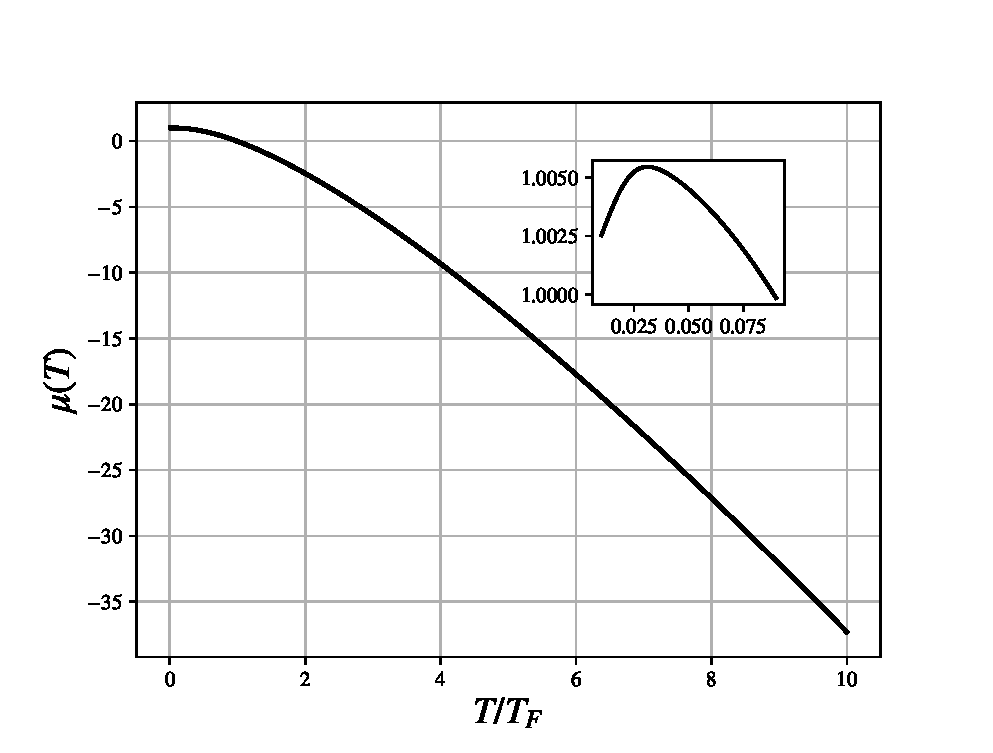
\includegraphics[scale=0.7]{scripts/mu_T.eps}
    \caption{Chemical potential as a function of temperature. The small window on top right is a zoom on the low-temperature area. It shows that for low temperature
    the chemical potential dependence on the temperature can be well approximated by a parabola of the type $\mu(T) = \mu(T=0) - \alpha T^2 = \epsilon_F - \alpha T^2$}
    \label{fig:chemical_potential}
\end{figure}

\subsubsection*{(d)}
The curves are already reported in figure \ref{fig:fFD_mu} as dashed lines, but I report them here alone for clarity
\begin{figure}
    \centering
    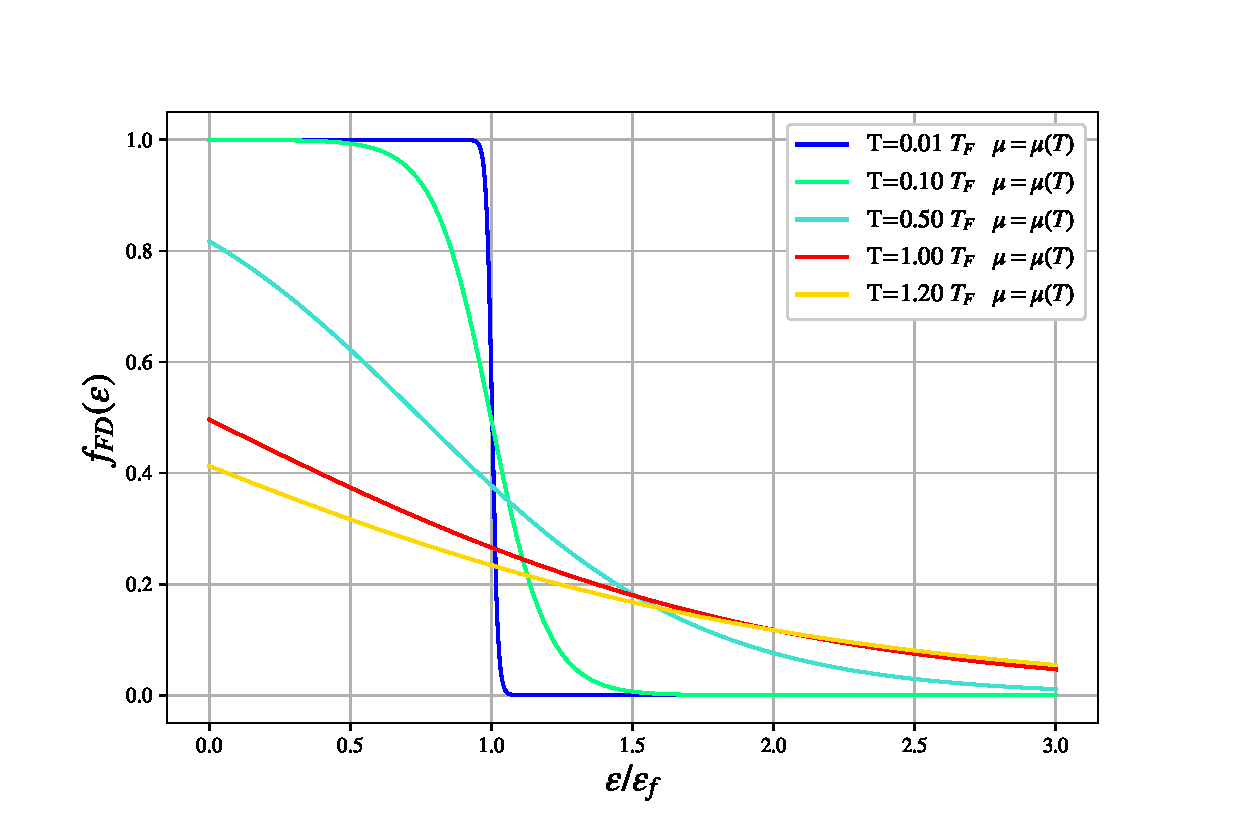
\includegraphics[scale=0.5]{scripts/f_fd_mu_T.eps}
    \caption{Fermi-Dirac distribution for various value of temperature. The depence of the chemical $\mu$ on the temperature is taken into account.}
    \label{fig:fFD_mu_T}
\end{figure}

\subsubsection*{(e)}
The energy of the system can be computed as 
\begin{equation*}
    E = \int_0^{+\infty} DOS(\epsilon) \, f_{FD}(\epsilon, T) \, \epsilon \, d\epsilon
\end{equation*}
The electrons' heat capacity contribution is
\begin{equation*}
    C = \frac{dE}{dT} = \int_0^{+\infty} DOS(\epsilon) \, \frac{\partial f_{FD}(\epsilon, T)}{\partial T} \, \epsilon \, d\epsilon
\end{equation*}
Since the number of electrons is independent of the temperature the last expression is equivalent to 
\begin{equation*}
    C = \frac{dE}{dT} - \epsilon_F\frac{dN}{dT} = \int_0^{+\infty} DOS(\epsilon) \, \frac{\partial f_{FD}(\epsilon, T)}{\partial T} \, (\epsilon -\epsilon_F) \, d\epsilon
\end{equation*}
Let us now consider the quantum limit $k_BT \ll \epsilon_F$: it can be easilly seen from figure (REFFF) that $\frac{df_{FD}}{d\epsilon}$ is significantly different from zero only 
in a small region of width $2k_BT$ centered in $\epsilon=\epsilon_F$. Hence
\begin{equation*}
    C \approx DOS(\epsilon_F) \int_0^{+\infty} \frac{\partial f_{FD}(\epsilon, T)}{\partial T} \, (\epsilon - \epsilon_F) \, d\epsilon = 
    DOS(\epsilon_F) k_B^2T \int_{-\epsilon_F/k_BT}^{+\infty} \frac{e^x}{(e^x + 1)^2} \, dx 
\end{equation*}
where I made the change of variable $x=(\epsilon - \epsilon_F)/k_BT$ and I used the fact that 
\begin{equation*}
    \frac{\partial f_{FD}(\epsilon, T)}{\partial T} = \frac{\epsilon - \epsilon_F}{k_BT^2} \frac{exp((\epsilon - \epsilon_F)/k_BT)}{[exp((\epsilon - \epsilon_F)/k_BT) + 1]^2}
\end{equation*}
that is I used the approximation $\mu \approx \epsilon_F$ (valid for the low temperature range).
Since we assumed $k_BT \ll \epsilon_F$ the lower extrema can be approximated to $-\infty$. The integral is now a known integral and the value is $\pi^2/3$. Using the fact that 
$DOS(\epsilon_F) = \frac{3N}{2\epsilon_F}$ the estimated specific heat is 
\begin{equation*}
    C \approx \frac{\pi^2}{2} N k_B^2 \frac{T}{E_F} = \frac{\pi^2}{2} N k_B \frac{T}{T_F}
\end{equation*}

\section{Exercise II}
Let us first consider a simple delta potential $V(x) = V_0 \, \delta(x)$ and the Schroedinger equation 
\begin{equation*}
    -\frac{\hbar^2}{2m}\psi''(x) + V(x) \psi(x) = E \psi(x)
\end{equation*}
Let us integrate both members between $-\epsilon$ and $+\epsilon$ and let $\epsilon \to 0$, we obtain (in approximation for small $\epsilon$)
\begin{equation*}
    \lim_{\epsilon \to 0} -\frac{\hbar^2}{2m} \left(\psi'(\epsilon) - \psi'(-\epsilon)\right) + V_0\int_{-\epsilon}^{+\epsilon} \delta(x) \psi(x) = \lim_{\epsilon \to 0} 2\epsilon E \psi(0)
\end{equation*} 
or 
\begin{equation*}
    \psi'(0^+) - \psi'(0^-) = \frac{2mV_0}{\hbar^2}\psi(0)
\end{equation*}
This equation can be read as a condition on the discontinuity of the derivative of the function $\psi(x)$ across the $\delta$. \\
Now let us return to the Dirac delta comb potential $V(x) = \sum_{n=-\infty}^{+\infty} \delta(x+na)$. The potential is clearly periodic with period $a$. Hence
one can make use of the Bloch's theorem which states that the wavefunctions satisfy the conditions
\begin{equation*}
    \psi(x) = e^{iQx} u(x)
\end{equation*}
where $Q=\frac{2\pi}{na}$ and $u(x)$ satisfies in turn
\begin{equation*}
    u(x+na) = u(x)
\end{equation*}
One can now restrict the domain to $0<x<a$ and solve the problem in this interval, imposing then the Bloch condition to obtain the solution 
to the complete theorem. For $0<x<a$ the solution is a plane wave
\begin{equation*}
    \psi(x) = Ae^{ikx} + Be^{-ikx}
\end{equation*}
By using the Bloch's theorem one can relate the solution for $a<x<2a$
\begin{equation*}
    \frac{\psi(x)}{\psi(x+a)} = \frac{u(x)e^{iQx}}{u(x+a)e^{iQx}e^{iqa}} = e^{-iQa}
\end{equation*}
So that 
$\psi(x+a) = e^{iQa} \, \psi(x)$
Let us now impose the continuity of $\psi(x)$ and the discontinuity of $\psi'(x)$ on the edge between the two zones at $x=a$
$$\begin{cases}
    eq1
\end{cases}$$
which can be reduced
\begin{equation*}
    \cos(Qa) = \cos(ka) + \frac{V_0}{2ka} \sin(ka)
\end{equation*}
The admitted values of $k$ for the system are those that satisfy the above equation. The corresponding energies are then $E_k = \frac{\hbar^2k^2}{2m}$.
The last equation has solution only if $|cos(ka) + \frac{V_0}{2ka} \sin(ka)| < 1$. 
For $|cos(ka) + \frac{V_0}{2ka} \sin(ka)| > 1$ there are no solutions: this means that therethose $k-$vectors are admitted by the system, hence those energies are not admitted.


\end{document}